\question[15]  Julian trota 2 kilómetros al este, 4 kilómetros al norte y luego 7 kilómetros al oeste,
como se muestra en la figura \ref{fig:des_pitagoras_08}.

\begin{figure}[H]
    \begin{center}
        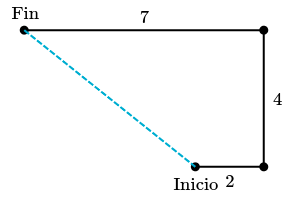
\includegraphics[width=0.4\textwidth]{../images/des_pitagoras_08.png}
    \end{center}
    \caption{}
    \label{fig:des_pitagoras_08}
\end{figure}

\textbf{¿Qué tan lejos está Julian de su posición inicial?}
\textit{Redondea tu respuesta a la décima de kilómetro más cercana.}
